\documentclass[journal]{IEEEtran}

\usepackage[T1]{fontenc}
\usepackage[utf8]{inputenc}
\usepackage{amsmath,amssymb,amsfonts}
\usepackage{graphicx}
\usepackage{booktabs}
\usepackage{array}
\usepackage{url}
\usepackage{xcolor}
\usepackage[hidelinks]{hyperref}
\usepackage{orcidlink}
\usepackage{balance}

\graphicspath{{../figures/}}

\renewcommand{\topfraction}{0.92}
\renewcommand{\bottomfraction}{0.75}
\renewcommand{\textfraction}{0.08}
\renewcommand{\floatpagefraction}{0.80}

% IEEEtran hard-codes an em-dash after the abstract and index-terms names; the CAOS
% content standard (ADR-0067) excludes em-dashes, so the separator is a full stop.
\makeatletter
\def\abstract{\normalfont
    \if@twocolumn
      \@IEEEabskeysecsize\bfseries\textit{\abstractname}.\ \relax
    \else
      \bgroup\par\addvspace{0.5\baselineskip}\centering\vspace{-1.78ex}\@IEEEabskeysecsize\textbf{\abstractname}\par\addvspace{0.5\baselineskip}\egroup\quotation\@IEEEabskeysecsize
    \fi\@IEEEgobbleleadPARNLSP}
\def\IEEEkeywords{\normalfont
    \if@twocolumn
      \@IEEEabskeysecsize\bfseries\textit{\IEEEkeywordsname}.\ \relax
    \else
      \bgroup\par\addvspace{0.5\baselineskip}\centering\@IEEEabskeysecsize\textbf{\IEEEkeywordsname}\par\addvspace{0.5\baselineskip}\egroup\quotation\@IEEEabskeysecsize
    \fi\@IEEEgobbleleadPARNLSP}
\makeatother

% Page-1 header block (conventions/manuscript-header-standard.md). The four document
% macros are set by the publishing tool when the version DOI is reserved.
\newcommand{\doctype}{Technical note}
\newcommand{\docversion}{v1.1}
\newcommand{\docdate}{18 September 2026}
\newcommand{\versiondoi}{10.5281/zenodo.22822959}
\newcommand{\conceptdoi}{10.5281/zenodo.21519891}
\newcommand{\docrepo}{github.com/fsantibanezleal/beltvision}
\newcommand{\headerblock}{%
\begin{center}
\fbox{\parbox{0.94\textwidth}{\small\raggedright
\textbf{\doctype} \quad$\cdot$\quad \docversion, \docdate \quad$\cdot$\quad Licence CC BY 4.0\\[2pt]
CAOS open-research programme \quad$\cdot$\quad \texttt{beltvision}, conveyor-belt inspection by computer vision\\[2pt]
Version DOI \href{https://doi.org/\versiondoi}{\texttt{\versiondoi}} \quad$\cdot$\quad
concept DOI (always latest) \href{https://doi.org/\conceptdoi}{\texttt{\conceptdoi}}\\[2pt]
Not peer reviewed. Source code, data and computational records: \href{https://\docrepo}{\texttt{\docrepo}}
}}
\end{center}}

\begin{document}

\title{beltvision: A Reproducible Classical\\ Computer-Vision Inspection Engine\\ for Conveyor Belts, Verified on\\ Ground-Truth Synthetic Scenes}

\author{Felipe~Santiba\~nez-Leal~\orcidlink{0000-0002-0150-3246}%
\thanks{F. Santiba\~nez-Leal is with the CAOS open-research programme, Santiago, Chile
(e-mail: fsantibanez@gmail.com; ORCID 0000-0002-0150-3246).}%
\thanks{Package \texttt{beltvision} (v0.11.3, Apache-2.0):
\url{https://github.com/fsantibanezleal/beltvision}.}}

\markboth{\doctype\ \docversion, 2026 \textperiodcentered\ CAOS open-research programme}%
{Santiba\~nez-Leal: beltvision, a reproducible classical-CV inspection engine for conveyor belts}

\IEEEaftertitletext{\vspace{-0.6\baselineskip}\headerblock\vspace{0.2\baselineskip}}

\maketitle

\begin{abstract}
Conveyor-belt inspection asks a vision system to find the belt, measure its geometry, tell an empty return
strand from a loaded one, and flag damage or foreign objects, and the practical difficulty is that most published
demonstrations run on private field footage that no one else can rerun. \texttt{beltvision} is a reusable
inspection engine that bundles the classical vision methods (CLAHE preprocessing, belt-edge geometry, semantic
layering, granulometry, anomaly and tracking) behind a staged pipeline, and it ships something a field demo
cannot: a deterministic suite of synthetic belt scenes carrying their exact ground truth, so the engine can be
benchmarked with no external or private data. This note reports that benchmark. On six generated scenes spanning
vertical, horizontal, diagonal, curved and laterally misaligned belts, the training-free classical chain recovers
the belt-axis orientation to a mean error of $2.5^\circ$ (worst $7.5^\circ$, all within the $8^\circ$ product
tolerance), recovers the belt footprint at a mean intersection-over-union of $0.81$, segments the exposed belt
rubber at $0.84$ and the mineral load at $0.96$, and recovers an injected lateral misalignment ($-9^\circ$ ground
truth) as $-7.47^\circ$, correct in sign and $1.53^\circ$ from the truth. The same ground truth also exposes a
limitation:
the classical core does not isolate small foreign objects (per-class intersection-over-union
$0.00$), which is exactly the task the engine delegates to an optional, lazily imported learned lane. Every number
regenerates from the seed and the released code; no belt imagery is redistributed.
\end{abstract}

\begin{IEEEkeywords}
computer vision, conveyor belt, inspection, image segmentation, anomaly detection, granulometry, reproducibility,
open-source software.
\end{IEEEkeywords}

\section{Introduction}

\IEEEPARstart{A} conveyor belt carrying ore is a continuous inspection problem: a camera over the belt should
locate the belt surface, measure its axis and alignment against the supporting structure, distinguish a loaded
top strand from an empty return strand, estimate the fragment-size distribution of the load, and raise a flag on a
rip, a hole or a tramp foreign object. Each of these has a mature classical-vision treatment, from CLAHE contrast
equalisation~\cite{clahe} through morphological granulometry~\cite{serra} to the deep anomaly-detection models
that now lead the industrial benchmarks~\cite{padim,patchcore}. The practical obstacle is not the methods; it is
that a belt-inspection demonstration is almost always shown on a private recording from one plant, which means the
numbers cannot be reproduced or compared by anyone else.

\texttt{beltvision} is built to remove that obstacle. It is a library, not an application and not a dataset: a
domain-agnostic inspection engine importable with a slim classical stack (\texttt{numpy}, \texttt{opencv},
\texttt{scikit-image}~\cite{skimage}, \texttt{scipy}), whose heavier deep-learning engines are optional extras
imported lazily and never at load time. Alongside the engine it ships a deterministic generator of synthetic belt
scenes that carry their \emph{exact} ground truth (the belt mask, the axis orientation, the medial-axis
centreline, the injected misalignment, a four-class label map and the injected damage and foreign-object boxes), so
the whole pipeline can run end to end and be scored against known geometry with no external data. This note reports
the benchmark that ground truth makes possible: how well the training-free classical chain recovers the belt
geometry and semantics, across orientations, and where it fails.

% Defined here so that the two-column float is placed at the top of page 2, beside Section III.
\begin{figure*}[!t]
\centering
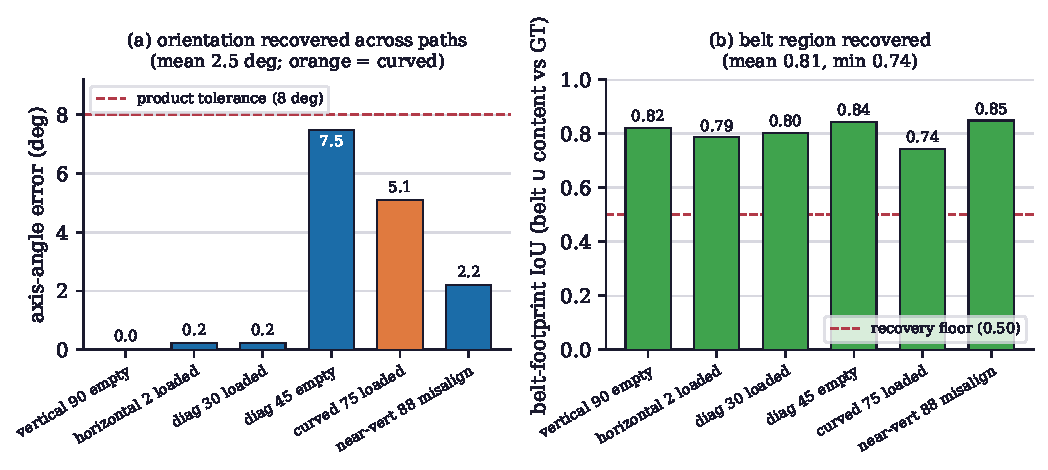
\includegraphics[width=0.92\textwidth]{fig-geometry.pdf}
\caption{The training-free classical chain (CLAHE, semantic layers, PCA axis, centreline, alignment) recovers the
known geometry of the synthetic suite. (a) Belt-axis orientation error per scene, against the $8^\circ$ product
tolerance; the two larger errors are the empty diagonal and the curved belt (orange), where a single straight
axis is an approximation by construction. (b) Belt-footprint intersection-over-union against the generated belt
mask, well above the $0.50$ recovery floor at every orientation.}
\label{fig:geometry}
\end{figure*}

\section{The Engine}\label{sec:engine}

The engine is a frozen six-stage pipeline (\texttt{preprocess}, \texttt{feature\_extraction}, \texttt{train},
\texttt{infer}, \texttt{evaluate}, \texttt{export}) whose stage signatures are stable while their bodies can be
replaced by heavier methods. Two data contracts bound it: an ingestion gate that accepts, flags or rejects
an input frame, and a validated artifact manifest that a viewer can replay without rerunning the pipeline. A
measured lane gate decides where a capability runs (in a browser, on a CPU server, or offline as a precompute
artifact) from measured bytes and milliseconds rather than a hand-assigned label. The classical methods
(preprocessing, belt-edge geometry, semantic layering, granulometry, tracking) run in the live lanes with the slim
stack; the learned anomaly detectors (a convolutional auto-encoder, PaDiM~\cite{padim} and
PatchCore~\cite{patchcore}, evaluated under the MVTec AD protocol~\cite{mvtec}) live behind the optional
\texttt{[dl]} extra and are imported only inside the precompute lane. This note benchmarks the classical core,
which is what runs without any model download or belt corpus.

\section{Ground-Truth Geometry Recovery}\label{sec:geometry}

The synthetic suite is six scenes chosen to break an all-vertical test: a vertical empty belt, a near-horizontal
loaded belt, diagonals at $30^\circ$ and $45^\circ$, a curved loaded belt, and a laterally misaligned belt. For
each, the classical chain segments the belt, fits its principal axis, traces the centreline and measures the axis
against the supporting structure, entirely training-free (\texttt{use\_learned=False}). Because the scene is
generated, the recovered geometry is compared to the exact truth.

Fig.~\ref{fig:geometry} reports the result. The belt-axis orientation is recovered to a mean error of $2.5^\circ$
across the whole orientation span, with three of the six scenes below $0.25^\circ$; the two larger errors,
$7.5^\circ$ on the empty $45^\circ$ diagonal and $5.1^\circ$ on the curved belt, are the expected cost of fitting a
single straight axis to a low-contrast or curved path, and both remain inside the $8^\circ$ tolerance
the product documents. The belt footprint, the belt-and-content region against the generated belt mask, is
recovered at a mean intersection-over-union of $0.81$ (minimum $0.74$ on the curved belt), comfortably above the
$0.50$ floor at every orientation. On the laterally misaligned scene, whose ground-truth belt-versus-support
misalignment is $-9^\circ$, the chain measures $-7.47^\circ$: correct in sign and $1.53^\circ$ from the truth,
the reading a belt-tracking alarm would key on. The whole classical chain runs in a mean of $71$~ms per frame on
one CPU core.

\section{Semantic Recovery and the Foreign-Object Limitation}\label{sec:semantic}

\begin{figure*}[!t]
\centering
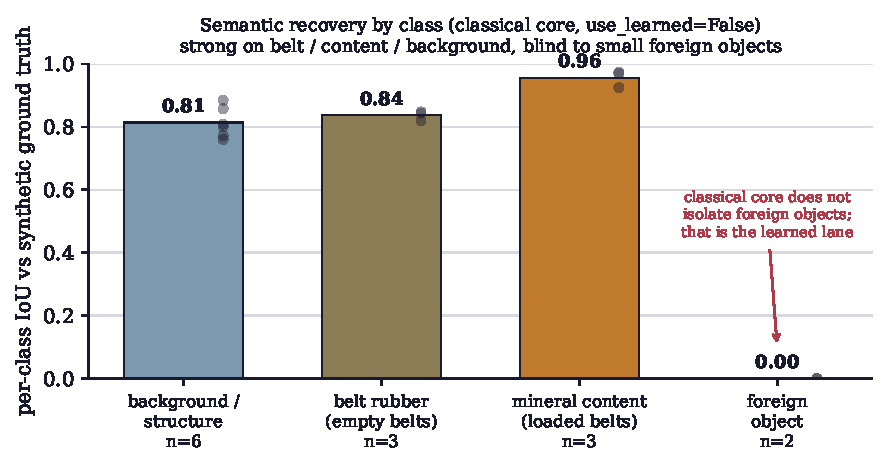
\includegraphics[width=0.78\textwidth]{fig-semantic.pdf}
\caption{Per-class segmentation of the classical core against the four-class synthetic ground truth, each class
scored where it is the observable surface. Background/structure, exposed belt rubber and mineral content are
recovered at intersection-over-union $0.81$ to $0.96$. Small foreign objects are not isolated by the classical
core (per-class intersection-over-union $0.00$): that class is the task the engine hands to its optional learned
lane. Dots are per-scene values.}
\label{fig:semantic}
\end{figure*}

The same ground truth carries a four-class label map (external structure, belt rubber, mineral content, foreign
object), so the semantic layering can be scored per class (Fig.~\ref{fig:semantic}). Scored where each class is the
exposed surface, the classical core recovers the background and support structure at intersection-over-union
$0.81$, the exposed belt rubber on empty belts at $0.84$, and the mineral load on loaded belts at $0.96$; on a
loaded belt the rubber is correctly relabelled as content rather than lost, which is why the belt class is scored
on the empty belts where the rubber is actually visible.

The fourth bar is a negative result. The classical core does not isolate the injected foreign objects: their
per-class intersection-over-union is $0.00$, because a small bright tramp object on a textured belt is not
separable by contrast and morphology alone, and the pixels fall into the surrounding content or belt class. This
is a limit of the method, not an implementation error, and it is the reason the engine keeps a learned anomaly
lane at all. The classical core is
the fast, dependency-light path that recovers belt geometry and coarse content, and the learned lane
(PaDiM~\cite{padim}, PatchCore~\cite{patchcore}, trained normal-only under the MVTec AD discipline~\cite{mvtec}) is
the path for the foreign-object and fine-anomaly task the classical core cannot do. The $0.00$ score is the
measured basis for that split.

\section{Scope and Reproduction}\label{sec:scope}

\texttt{beltvision} is a library other applications consume, not a service and not a
trained-model zoo; the bundled cases are a registry plus deterministic synthetic scenes, and real frames are
brought by the consumer. The benchmark here is therefore a \emph{geometry-recovery} benchmark on synthetic scenes
with known truth, not a field-performance claim on plant footage: it proves that the classical chain recovers
orientation, footprint, content and misalignment across orientations, and it locates the one class the classical
core cannot do. The learned anomaly lane is described but not benchmarked here, because a fair learned benchmark
needs a real belt corpus, which the library deliberately does not bundle or redistribute. Everything in
Fig.~\ref{fig:geometry} and Fig.~\ref{fig:semantic} regenerates from the seed and the released code:
\texttt{run\_bench.py} runs the synthetic suite through the classical chain and writes the measured errors, and
\texttt{make\_figs.py} renders the figures; no belt imagery is involved.

\section{Conclusion}

\texttt{beltvision} packages the classical conveyor-belt vision methods behind a staged, contract-bounded pipeline
and, unusually, ships the ground truth to test itself. On a six-scene synthetic suite spanning orientations, its
training-free classical core recovers belt orientation to $2.5^\circ$ mean error, the belt footprint to
intersection-over-union $0.81$, mineral content to $0.96$, and a $-9^\circ$ lateral misalignment with an error of
$1.53^\circ$, at $71$~ms per frame on a CPU. It also reports, from the same ground truth, that the classical
core cannot isolate small foreign objects, which is the task delegated to an optional learned lane. The note's
contribution is a reproducible, data-free benchmark of a real inspection engine that measures what the classical
path does and does not recover.

% \balance must be issued in the first column of the last page.
\balance

\appendices
\section{Reproduction}\label{app:repro}

{\raggedright
The benchmark output (\path{manuscripts/belt-inspection/data/bv.json}) carries, per scene, the ground-truth
and recovered belt orientation, the belt-footprint and per-class intersection-over-union, the measured
misalignment, the centreline root-mean-square error on straight belts, and the per-frame CPU time.
\path{figures/run_bench.py} produces it by running the ground-truth suite of \path{beltvision.cases.synthetic}
through \path{compute_layers} and \path{compute_belt_geometry} with \path{use_learned=False};
\path{figures/make_figs.py} renders both figures from it. The classical stack is
\texttt{numpy}/\texttt{opencv}/\texttt{scikit-image}/\texttt{scipy}; no model artifacts or belt corpus are needed
to reproduce any number in this note.\par}

\begin{thebibliography}{00}

\bibitem{clahe} K.~Zuiderveld, ``Contrast limited adaptive histogram equalization,'' in \emph{Graphics Gems IV},
P.~S. Heckbert, Ed. San Diego, CA, USA: Academic Press, 1994, pp.~474--485.

\bibitem{serra} J.~Serra, \emph{Image Analysis and Mathematical Morphology}. London, U.K.: Academic Press, 1982.

\bibitem{skimage} S.~van~der~Walt, J.~L. Sch\"onberger, J.~Nunez-Iglesias, F.~Boulogne, J.~D. Warner, N.~Yager,
E.~Gouillart, and T.~Yu, ``scikit-image: image processing in Python,'' \emph{PeerJ}, vol.~2, art.~e453, 2014.
doi:10.7717/peerj.453.

\bibitem{mvtec} P.~Bergmann, M.~Fauser, D.~Sattlegger, and C.~Steger, ``MVTec AD: A comprehensive real-world
dataset for unsupervised anomaly detection,'' in \emph{Proc. IEEE/CVF Conf. Comput. Vis. Pattern Recognit.
(CVPR)}, 2019, pp.~9592--9600. doi:10.1109/CVPR.2019.00982.

\bibitem{padim} T.~Defard, A.~Setkov, A.~Loesch, and R.~Audigier, ``PaDiM: A patch distribution modeling framework
for anomaly detection and localization,'' 2020. arXiv:2011.08785.

\bibitem{patchcore} K.~Roth, L.~Pemula, J.~Zepeda, B.~Sch\"olkopf, T.~Brox, and P.~Gehler, ``Towards total recall
in industrial anomaly detection,'' 2021. arXiv:2106.08265.

\end{thebibliography}

\end{document}
